% SROD analysis report -- reference version. Build: pdflatex SROD_ANALYSIS_REPORT.tex (twice).
% docs/SROD_ANALYSIS_REPORT.md and the published HTML page mirror this file.
\documentclass[11pt,a4paper]{article}
\usepackage[margin=25mm]{geometry}
\usepackage[T1]{fontenc}
\usepackage[utf8]{inputenc}
\usepackage{lmodern}
\usepackage{amsmath}
\usepackage{amssymb}
\usepackage{booktabs}
\usepackage{graphicx}
\usepackage{siunitx}
\usepackage{caption}
\usepackage{enumitem}
\usepackage{listings}
\usepackage[hidelinks]{hyperref}
\sisetup{range-phrase=--,range-units=single,per-mode=symbol,detect-all}
\captionsetup{font=small,labelfont=bf}
\lstset{basicstyle=\ttfamily\small,breaklines=true,columns=fullflexible,frame=single,framesep=4pt}
\graphicspath{{./}}
\setlist{nosep}
\emergencystretch=0.15\textwidth

\newcommand{\code}[1]{\texttt{#1}}
\newcommand{\dir}[1]{$\langle #1 \rangle$}
\newcommand{\Dunit}{\si{deg\squared\per\micro\metre}}

\title{Misorientation accumulation along columnar grains in GammaPrint-700 laser powder bed fusion:\\ 3D-EBSD (Lamb et al.) versus SPPARKS}
\author{SURGE-kokkos branch, \code{additive/texture/kk} Moser deck}
\date{Status 2026-09-09}

\begin{document}
\maketitle

\begin{abstract}
Lamb et al.\ measured the starting reference orientation deviation (SROD) of columnar grains in a 3D-EBSD volume of laser powder bed fusion GammaPrint-700. Re-analysing their Fig.~5 shows that the population SROD is a random-axis rotation walk: $\mathrm{RMS}^2 = D h$ with $D \approx \SI{0.42}{\Dunit}$ against build height, the same $D$ for grains originating inside the volume and for established grains, and a 5/95 band of $(p_{95}-p_5)/\text{mean} \approx 1.4$, the Maxwell width of a three-dimensional walk. Their Fig.~4 shows that individual grains rotate coherently along a directed path. SPPARKS \code{additive/texture} and \code{additive/texture/kk} now carry a two-term model: a per-voxel walk of angle $\sqrt{D_v\,\mathrm{hop}}$ inherited along each lineage, and a coherent per-grain walk of the rotation vector, indexed by the inheritance path length and correlated between levels (Ornstein--Uhlenbeck), shared by every voxel of the grain. A Moser-source GP700 deck with this model reproduces the experiment on both levels: population SROD RMS deviation from Lamb's mean \SI{0.34}{\degree} over \SIrange{25}{240}{\micro\metre}, bias \SI{-0.28}{\degree}, band/mean 1.50, and per-grain drifts of 8--\SI{15}{\degree} over \SI{400}{\micro\metre} with a 3--\SI{7}{\degree} intragranular spread. Two model corrections were required along the way, per-grain parent selection and copy-mode boundary smoothing. The deck constants are per unit of growth path, which is $1.8\times$ the height in this remelt geometry, and are resolution independent to first order. Open issues: the simulated grains are epitaxial substrate continuations, so Lamb's originating class is essentially absent; the split between the coherent and per-voxel terms and the correlation height are constrained only loosely by the published data; the \dir{001} fibre has no quantitative target.
\end{abstract}

\section{Summary}
\begin{itemize}
\item Population SROD in GP700 is a rotation walk, $D \approx \SI{0.42}{\Dunit}$ against height, Maxwell width; both grain classes obey it. Individual grains rotate coherently along a directed path (Lamb Fig.~4).
\item Model, both SPPARKS additive apps: \code{misorientation\_diffusion} $D_v$ (per-voxel walk, inherited per hop) plus \code{misorientation\_grain\_walk} $D_g$ $\rho$ \code{path} (coherent per-grain walk, one Gaussian rotation-vector increment per unit of inheritance path length, correlated between levels with persistence $\rho$). The path length is a per-site field (d10). Orientation is inherited from one parent voxel and never averaged: per-grain parent selection and copy-mode smoothing are part of the model.
\item Calibrated deck (\code{examples/gp700\_moser/}, build v10): $D_v$ \SI{0.065}{\Dunit}, $D_g$ \SI{0.010}{\Dunit}, $\rho = 0.9$ (correlation length $\approx \SI{30}{\micro\metre}$ of path). Against Lamb: RMS \SI{0.34}{\degree}, bias \SI{-0.28}{\degree}, band/mean 1.50 (Table~\ref{tab:v10}); per-grain drift median \SI{7.2}{\degree}, spread \SI{3.4}{\degree} (Table~\ref{tab:grains}).
\item The constants are per unit of growth path, $1.8\times$ the height here, and first-order resolution independent: the same deck reproduces Lamb at the experiment's \SI{1.5}{\micro\metre} voxel (bias \SI{+0.41}{\degree}).
\item Open: no surviving grains originate mid-build (83 of 88 filtered grains start at the first remelt floor); $D_g : D_v$ and $\rho$ need Lamb's within-slice widths and their population curve below \SI{30}{\micro\metre}; the \dir{001} fibre (0.15--0.19 within \SI{15}{\degree} of BD) has no measured target.
\end{itemize}

\section{Experimental methods (Lamb et al.\ 2023, Met.\ Trans.\ A 2026)}
\paragraph{Material and process.} CoNi-base superalloy GammaPrint-700, laser powder bed fusion at \SI{176}{\watt} and \SI{1137}{\milli\metre\per\second}, \SI{80}{\micro\metre} spot ($D4\sigma$), \SI{80}{\micro\metre} hatch, \SI{30}{\micro\metre} layers, \SI{90}{\degree} interlayer rotation, \SI{200}{\celsius} plate preheat. The 2026 paper supplies the thermophysical set used for its 3DThesis simulations: $k = \SI{22.5}{\watt\per\metre\per\kelvin}$, $\rho = \SI{8650}{\kilogram\per\cubic\metre}$, $c_p = \SI{600}{\joule\per\kilogram\per\kelvin}$ ($\alpha = \SI{4.335e-6}{\metre\squared\per\second}$), absorptivity 0.9, liquidus \SI{1646}{\kelvin}, solidus \SI{1592}{\kelvin}.

\paragraph{3D dataset.} TriBeam tomography (femtosecond-laser serial sectioning with EBSD on each slice), \SI{1.5}{\micro\metre} in-plane step and \SI{1.5}{\micro\metre} slice thickness, 385 slices, reconstructed into one HDF5 volume and segmented into grains at a \SI{2}{\degree} misorientation threshold before any SROD calculation.

\paragraph{SROD.} For each grain the reference orientation sits near the origination point, ``the lowest location of a grain's boundary along the build direction'', offset one voxel layer (\SI{1.5}{\micro\metre}) upward so the reference is not a boundary pixel with a convoluted EBSD pattern; offsets up to \SI{8}{\micro\metre} do not change the result. Two classes: \emph{originating} grains, whose lowest point lies inside the volume, and \emph{established} grains, cut by the dataset floor and referenced at the centroid of their footprint on the lowest slice. Grains shorter than \SI{60}{\micro\metre} (two layers) or under \SI{40}{\micro\metre} equivalent spherical diameter (ESD) are excluded as overtaken during competitive growth, leaving over 500 originating and over 100 established grains. Each grain is sliced along the build direction; each slice gives a SROD histogram fitted to a normal distribution and plotted against height above the origin (Fig.~5a) or above the dataset floor (Fig.~5c). Fig.~4 follows four individual grains with IPF and SROD maps, the mean SROD per layer, and every voxel on the build-direction inverse pole figure, where an arrow marks the rotation path from bottom to top; one grain splits into two orientation clusters. The 2026 paper adds that cells switch \dir{100} growth variants at fusion lines rather than rotating continuously, so no gradient-directed rotation is modelled.

\section{Analysis of the experimental data}
Fig.~5a and 5c were digitized from \SI{300}{dpi} renders of the paper (\code{docs/srod\_random\_walk.py}; curves in \code{docs/lamb2023\_fig5\{a,c\}\_srod.json}). The mean, 5th and 95th percentile curves were tested against a rotation walk: each increment is a small rotation of angle $\theta$ about a random axis; after $n$ independent increments the misorientation from the origin has
\begin{equation}
\mathrm{RMS}^2 = n\,\theta^2 = D\,d
\end{equation}
and a Maxwell distribution ($\chi$ with three degrees of freedom), for which $(p_{95}-p_5)/\text{mean} = 1.38$ at every distance. $D = \SI{0.42}{\Dunit}$ fitted on the originating grains predicts the established grains without refitting; the measured width ratio is 1.3--1.5 at every height; the apparent two-regime shape is the square root (Fig.~\ref{fig:exp}). A constant per-hop angle is not required, only independent increments with finite variance. The population statistics do not distinguish whether the increments belong to individual voxel lineages or to whole grains: each grain's coherent walk is one realisation, and the Maxwell width appears across grains either way. Fig.~4 supplies that missing information: the grains' mean orientation moves along a path, so the accumulation is at least partly coherent across the grain.

\begin{figure}[htbp]
\centering
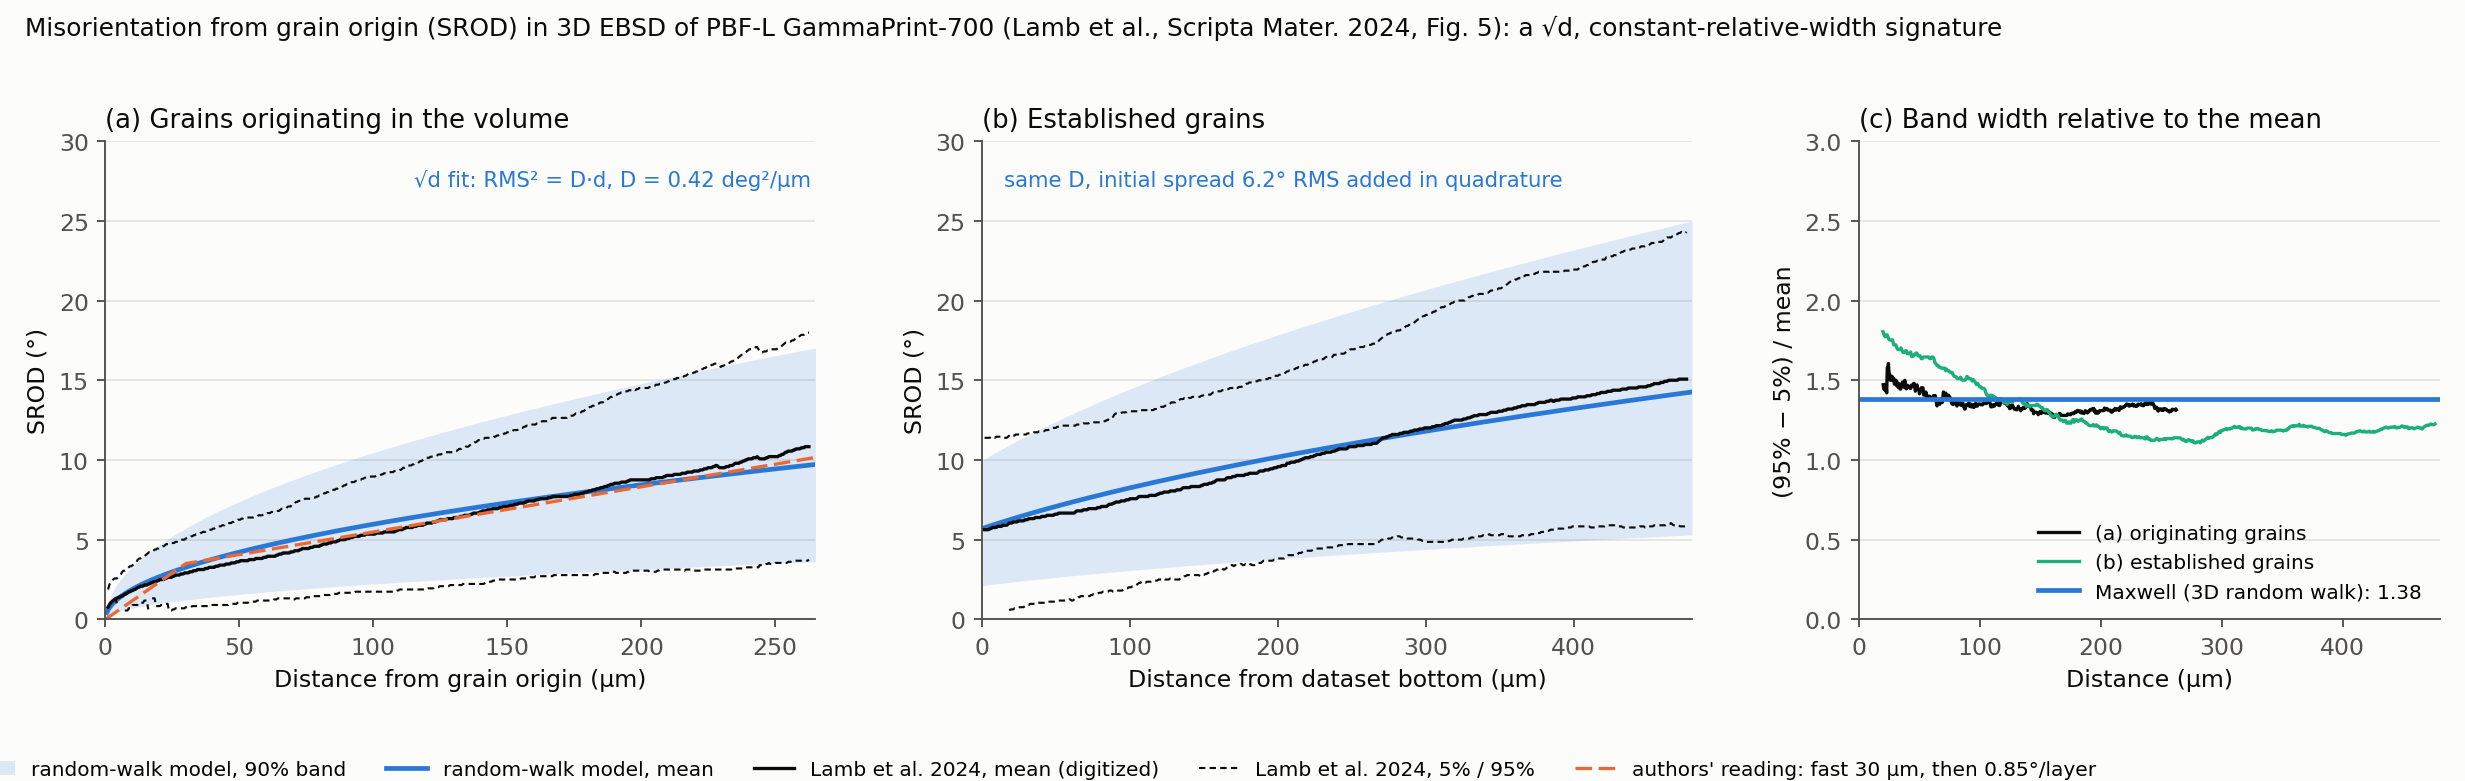
\includegraphics[width=\textwidth]{srod_experimental_analysis.png}
\caption{Lamb 2023 Fig.~5 digitized. Left: mean SROD of originating grains with $\mathrm{RMS}^2 = D h$, $D = \SI{0.42}{\Dunit}$; the same $D$ drawn through the established grains. Right: $(p_{95}-p_5)/\text{mean}$ against height, flat at 1.3--1.5 around the Maxwell value 1.38.}
\label{fig:exp}
\end{figure}

\section{Simulation methods}
\paragraph{Code.} SPPARKS, branch SURGE-kokkos, app \code{additive/texture/kk} (Kokkos/HIP on an AMD gfx1151 APU), one MPI rank. The CPU app \code{additive/texture} carries the same model and is the correctness reference; the temperature field is deterministic and bit-identical between the two (\code{examples/am\_validation/}).

\paragraph{Thermal source.} Moser Green's-function solution with the GP700 constants (\code{setup\_temperature\_source moser 176 0.9 22.5 4.335e-6 473 600 20e-6 20e-6 10e-6}), evaluated on the device for every site each step. Scan lines with \code{hatch 80e-6 N serpentine pause 8.8e-3}, the pause being the real \SI{10}{\milli\metre} track length over the scan speed; the fast-forward predictor skips idle gaps. Single-hatch check: pool $147 \times 69$~\si{\micro\metre}, thermal gradient \SIrange{1e7}{2.9e7}{\kelvin\per\metre} at the fusion boundary (paper: \SI{3e7}{\kelvin\per\metre}).

\paragraph{Build.} Box-per-layer stitch continuation (\code{run\_layers.sh}). Domain \SI{801}{\micro\metre} square (267 voxels at \SI{3}{\micro\metre}), 10 hatches at $40 + 80k$ \si{\micro\metre} with lines \SI{100}{\micro\metre} past both edges, 12 layers of \SI{30}{\micro\metre}, \SI{90}{\degree} rotation per layer, each box a \SI{180}{\micro\metre} window below the laser plane; each layer starts from the preheat (the recoat interval). Substrate: \SI{150}{\micro\metre} of \SI{50}{\micro\metre} Voronoi grains with uniform random orientations (\code{make\_substrate.py}); five overlapping hatches remelt \SIrange{80}{100}{\micro\metre}, so the analysable volume begins at \SI{105}{\micro\metre}. Timestep \SI{4}{\micro\second}, twice the $\Delta x / V(T_l - T_s)$ guard; 2 and \SI{4}{\micro\second} agree within seed noise. Calibration used a \SI{600}{\micro\metre}, 7-hatch, 8-layer proxy at \SI{3}{\minute} of loop time per box.

\paragraph{Solidification kinetics.} Front velocity is the 304L polynomial $\times 3.5$ (front at \SIrange{25}{35}{\kelvin} undercooling, about \SI{0.56}{\metre\per\second}, keeping up with the \SI{1.137}{\metre\per\second} scan); nucleation density \SI{1.5e13}{\per\cubic\metre}, critical undercooling \SI{15}{\kelvin}, deviation \SI{2}{\kelvin}. Parent selection per grain: candidate neighbours are grouped by grain, each grain weighted by the mobility $1 + c_2 \cos(c_3 \theta)$ of its sign-aligned mean orientation against the local thermal gradient ($c_2 = 2.8$, $c_3 = 2.5$, negative clamped to zero), then the parent voxel is drawn uniformly inside the chosen grain. Weighting among the voxels of one grain instead rotated grains toward \dir{001} with height and is not used.

\paragraph{Misorientation model.} Two terms, both applied at capture in the sample frame.
\begin{itemize}
\item \emph{Per-voxel walk}, \code{misorientation\_diffusion} $D_v$ \code{30}: the captured voxel takes its parent's orientation rotated by $\theta = \sqrt{D_v\,\mathrm{hop}}$ about a random axis (hop = lattice distance to the parent). A rotation past \SI{30}{\degree} would start a new grain (never reached). Independent lineages of one grain diverge, so this term supplies intragranular spread and no net drift.
\item \emph{Coherent grain walk}, \code{misorientation\_grain\_walk} $D_g$ $\rho$ \code{path}: every voxel carries its inheritance path length $s$ in lattice units (per-site field d10: zero at melt and at nuclei, parent plus hop at capture, copied with the orientation on a smoothing flip, exchanged with ghosts and continued through the stitch). Between path levels $k$ and $k+1$ every voxel of grain $g$ receives the same rotation, a Gaussian rotation vector $v_k$ of RMS $\sqrt{D_g \Delta x}$ whose sequence in $k$ is Ornstein--Uhlenbeck, $v_k = \rho\,v_{k-1} + \sqrt{1-\rho^2}\,v'_k$, with $v'_k$ hashed from $(g, k)$ so the sequence is a pure function of grain and level, path independent and without stored state; the correlation length is $\approx \Delta x/(1-\rho)$ of path and the long-range accumulation is $D_g (1+\rho)/(1-\rho)$ per unit path. This term supplies the coherent drift. A device cache of the recurrence (16384 grains $\times$ 768 levels) makes the term cost nothing measurable; grains or levels beyond it fall back to the direct evaluation.
\end{itemize}
\code{height} in place of \code{path} indexes the coherent walk by the lattice $z$ level instead; it is kept for comparison and is not used.

\paragraph{Boundary smoothing.} One greedy steepest-descent pass per captured voxel (\code{smooth\_greedy\_multiproposal on}, nrefine 1) the step after capture, and \code{smooth\_orientation copy}: a voxel that changes grain takes one random neighbour's orientation and path length from that grain. The default \code{average} (sign-aligned mean of the new grain's neighbours) cancels the fresh rotations of a voxel-scale mixed front, retains only 0.3--0.45 of the input $D$ and widens the population band to 1.8; it is not used.

\section{Simulation analysis methods}
\code{gp700\_analysis.py} on the spparks-micro-analysis tools: read the last stitch frame; solid means \code{i2 == 3}, so unremelted substrate is excluded; crop to the central \SI{400}{\micro\metre} laterally (\SI{300}{\micro\metre} on the proxy); relabel grains as connected components of spin; grain volume, ESD and extents; Lamb's filters (height $\geq \SI{60}{\micro\metre}$, ESD $\geq \SI{40}{\micro\metre}$); origin = the grain's lowest solid voxel, whose quaternion is the reference (exact in the simulation, so no offset); grains crossing the analysis floor are established and referenced at their floor-slice centroid. SROD is the symmetry-reduced disorientation of every voxel from its grain's reference, binned by height above the origin or floor in \SI{10}{\micro\metre} steps with mean, $p_5$, $p_{95}$ and RMS per bin. Score: RMS of (simulated mean $-$ Lamb Fig.~5a mean) over \SIrange{25}{240}{\micro\metre}, plus bias, $(p_{95}-p_5)/\text{mean}$, the fraction of solid within \SI{15}{\degree} of \dir{001} parallel to the build direction, and grain counts. Sobol designs (scipy \code{qmc}) on the proxy were used for calibration.

\code{grain\_paths.py} reproduces Lamb's Fig.~4 per grain and extends it to every filtered grain: IPF-Z and SROD maps on the $xz$ slice through the grain, mean SROD per \SI{10}{\micro\metre} slab, the per-slab mean orientation as a path on the build-direction inverse pole figure, the drift of the mean orientation from the bottom three slabs to the top three, the RMS spread of the top slabs about their mean, the maximum SROD, and the fraction of slabs in which the mean SROD rises.

\section{Results}
\subsection{Calibration path}
\begin{table}[htbp]
\centering\small
\caption{Full builds against Lamb Fig.~5a (all-originating SROD, central \SI{400}{\micro\metre} crop).}
\label{tab:path}
\resizebox{\textwidth}{!}{%
\begin{tabular}{llrrr}
\toprule
build & model & RMS / bias vs Lamb & band/mean & per-grain drift / spread (median) \\
\midrule
v2 & per-voxel walk, $D_v$ 0.42, voxel-level parent selection & \SI{2.2}{\degree} / \SI{+3.6}{\degree} (linear growth) & 1.4--1.8 & -- \\
v5 & per-grain parent selection, average smoothing, $D_v$ 1.15 & \SI{0.59}{\degree} / \SI{-0.16}{\degree} & 1.79 & -- \\
v8 & copy smoothing, $D_v$ 0.22 & \SI{0.49}{\degree} / \SI{+0.17}{\degree} & 1.41 & 4.2 / \SI{6.1}{\degree} \\
\textbf{v10} & \textbf{+ coherent path walk $D_g$ 0.010, $\rho$ 0.9; $D_v$ 0.065} & \textbf{\SI{0.34}{\degree} / \SI{-0.28}{\degree}} & \textbf{1.50} & \textbf{7.2 / \SI{3.4}{\degree}} \\
\bottomrule
\end{tabular}}
\end{table}

v2's linear growth was selection drift among the voxels of one grain. v5 to v7 retained only 0.3--0.45 of the input $D$ against height and had a 1.8 band, both from the averaging smoothing rule; copy-mode smoothing (v8) put the population curve, shape and band on Lamb. v8's grains, however, spread without drifting: the per-voxel walk lets the lineages of one grain diverge independently, so the cloud on the inverse pole figure expands about a stationary mean, whereas Lamb's grains move along a path. The coherent grain walk (v10) supplies the drift. A memoryless coherent walk makes individual SROD($h$) curves wander; correlating the rotation vector between levels ($\rho$) makes them rise along a directed path, and with Gaussian increments the population band stays at Lamb's value in both the ballistic and the diffusive regime. Indexing the coherent walk by path length rather than height removes the build-direction assumption, gives the AR(1) amplification exactly, and produces an intragranular spread from path dispersion alone.

\subsection{v10 against Lamb}
\begin{table}[htbp]
\centering\small
\caption{v10: $D_v$ \SI{0.065}{\Dunit}, $D_g$ \SI{0.010}{\Dunit}, $\rho$ 0.9 path, copy smoothing, nrefine 1, Voronoi substrate, nucleation \SI{1.5e13}{\per\cubic\metre}, $t_c$ \SI{15}{\kelvin}, $c_2$ 2.8, $\Delta t$ \SI{4}{\micro\second}, \SI{3}{\micro\metre}.}
\label{tab:v10}
\resizebox{\textwidth}{!}{%
\begin{tabular}{lrrr}
\toprule
 & v10 & v8 (per-voxel only) & Lamb 2023 \\
\midrule
SROD RMS deviation, \SIrange{25}{240}{\micro\metre} & \SI{0.34}{\degree} & \SI{0.49}{\degree} & -- \\
mean bias & \SI{-0.28}{\degree} & \SI{+0.17}{\degree} & -- \\
mean SROD at 54 / 204 / \SI{402}{\micro\metre} & 3.6 / 8.2 / \SI{12.1}{\degree} & 4.4 / 8.5 / \SI{12.3}{\degree} & 3.8 / 8.8 / -- (data end at \SI{262}{\micro\metre}) \\
$(p_{95}-p_5)/\text{mean}$ & 1.50 & 1.41 & 1.4 \\
$D$-fit vs height & \SI{0.43}{\Dunit} & \SI{0.41}{\Dunit} & 0.42 \\
grains passing filters (\SI{400}{\micro\metre} crop) & 97 & 86 & $>600$ (full volume) \\
ESD $p_{10}$ / $p_{50}$ / $p_{90}$ & 76 / 148 / \SI{170}{\micro\metre} & 73 / 151 / \SI{182}{\micro\metre} & -- \\
\dir{001} within \SI{15}{\degree} of BD & 0.15 & 0.19 & qualitative \dir{001} fibre \\
\bottomrule
\end{tabular}}
\end{table}

\begin{figure}[htbp]
\centering
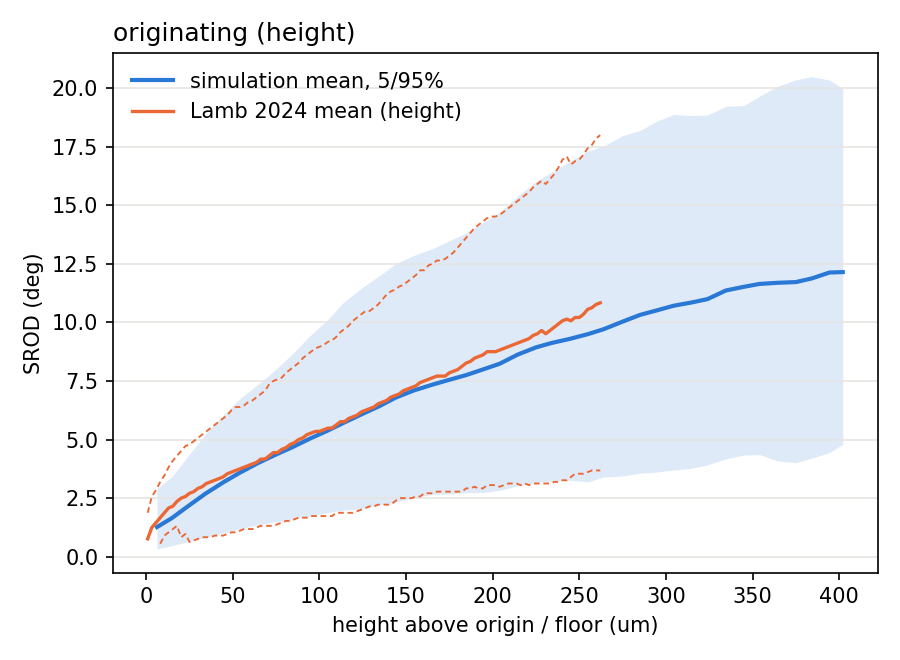
\includegraphics[width=0.75\textwidth]{gp700_results_v10/srod_height.png}
\caption{v10, all-originating SROD against height above the origin (central \SI{400}{\micro\metre} crop, floor \SI{100}{\micro\metre}): simulated mean with the 5/95 band (blue) against Lamb 2023 mean and percentiles (orange).}
\label{fig:v10srod}
\end{figure}

\begin{figure}[htbp]
\centering
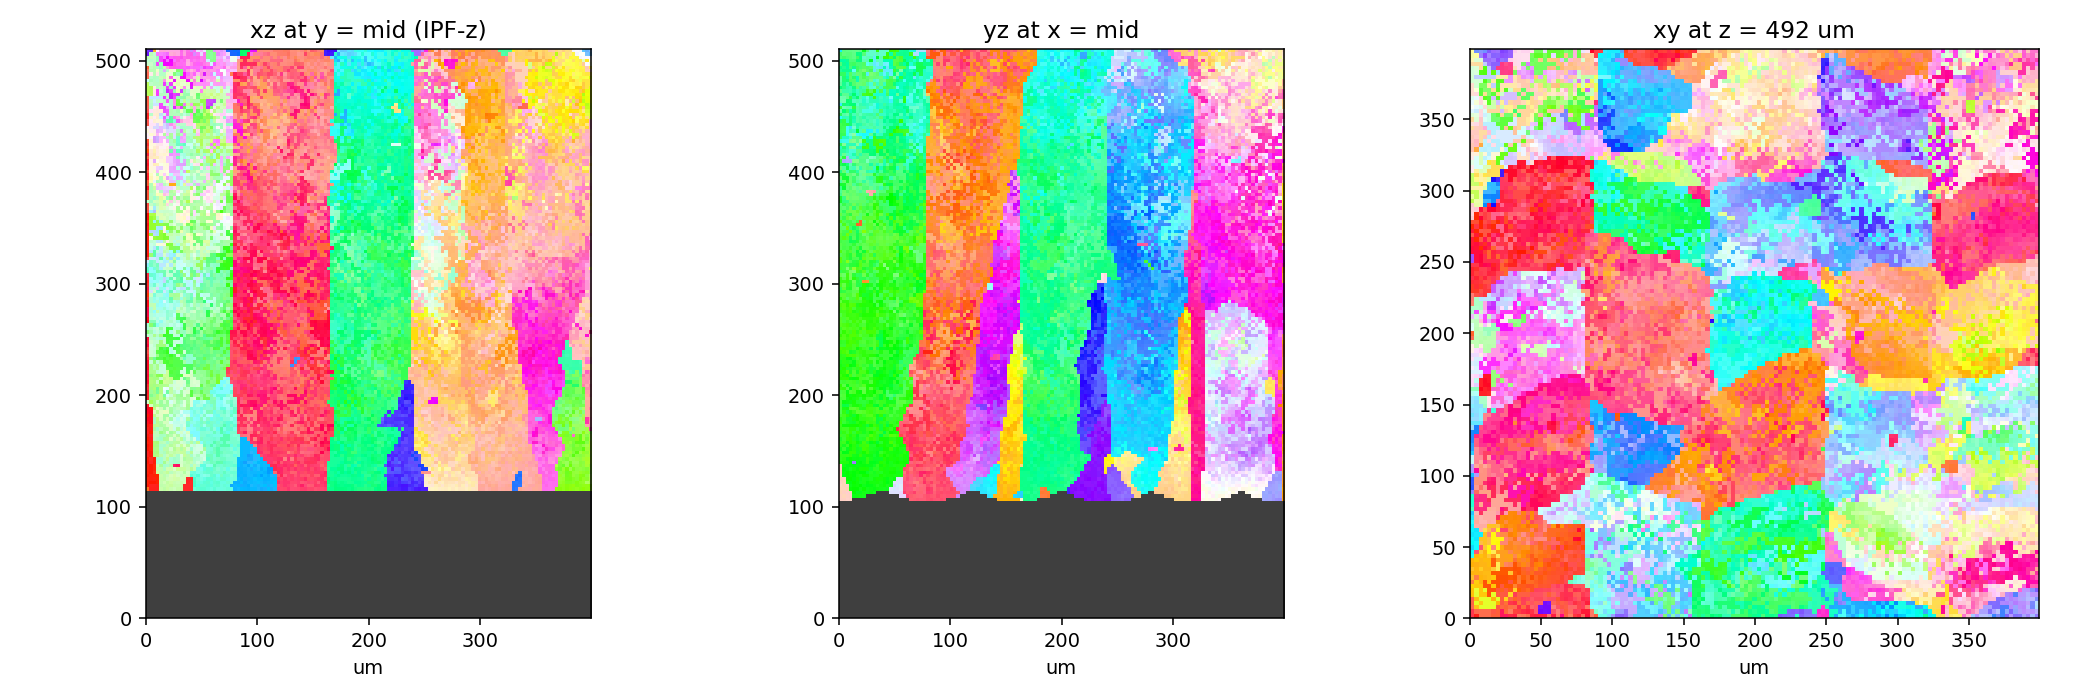
\includegraphics[width=\textwidth]{gp700_results_v10/ipf_sections.png}
\caption{v10 IPF-Z colouring: $xz$ and $yz$ sections through the crop centre, and the $xy$ section at \SI{492}{\micro\metre}. Dark grey is the unremelted substrate.}
\label{fig:v10ipf}
\end{figure}

\subsection{Per-grain orientation paths}
\begin{table}[htbp]
\centering\small
\caption{Every filtered grain of the two full builds (\code{grain\_paths.py}): drift of the mean orientation from the bottom three \SI{10}{\micro\metre} slabs to the top three, RMS spread of the top slabs about their mean, maximum SROD, and the fraction of slabs in which the mean SROD rises. Medians, with $p_{10}$ / $p_{90}$ for the drift.}
\label{tab:grains}
\begin{tabular}{lrr}
\toprule
 & v10 (96 grains) & v8 (86 grains) \\
\midrule
drift of the mean, bottom $\to$ top & \SI{7.2}{\degree} (1.7 / 13.5) & \SI{4.2}{\degree} (2.0 / 7.5) \\
spread about the top-slab mean & \SI{3.4}{\degree} & \SI{6.1}{\degree} \\
drift $\div$ spread & 1.66 & 0.60 \\
maximum SROD in the grain & \SI{15.0}{\degree} & \SI{16.0}{\degree} \\
top-slab mean SROD & \SI{8.4}{\degree} & \SI{8.2}{\degree} \\
fraction of slabs with rising mean SROD & 0.79 & 0.78 \\
\bottomrule
\end{tabular}
\end{table}

\begin{figure}[htbp]
\centering
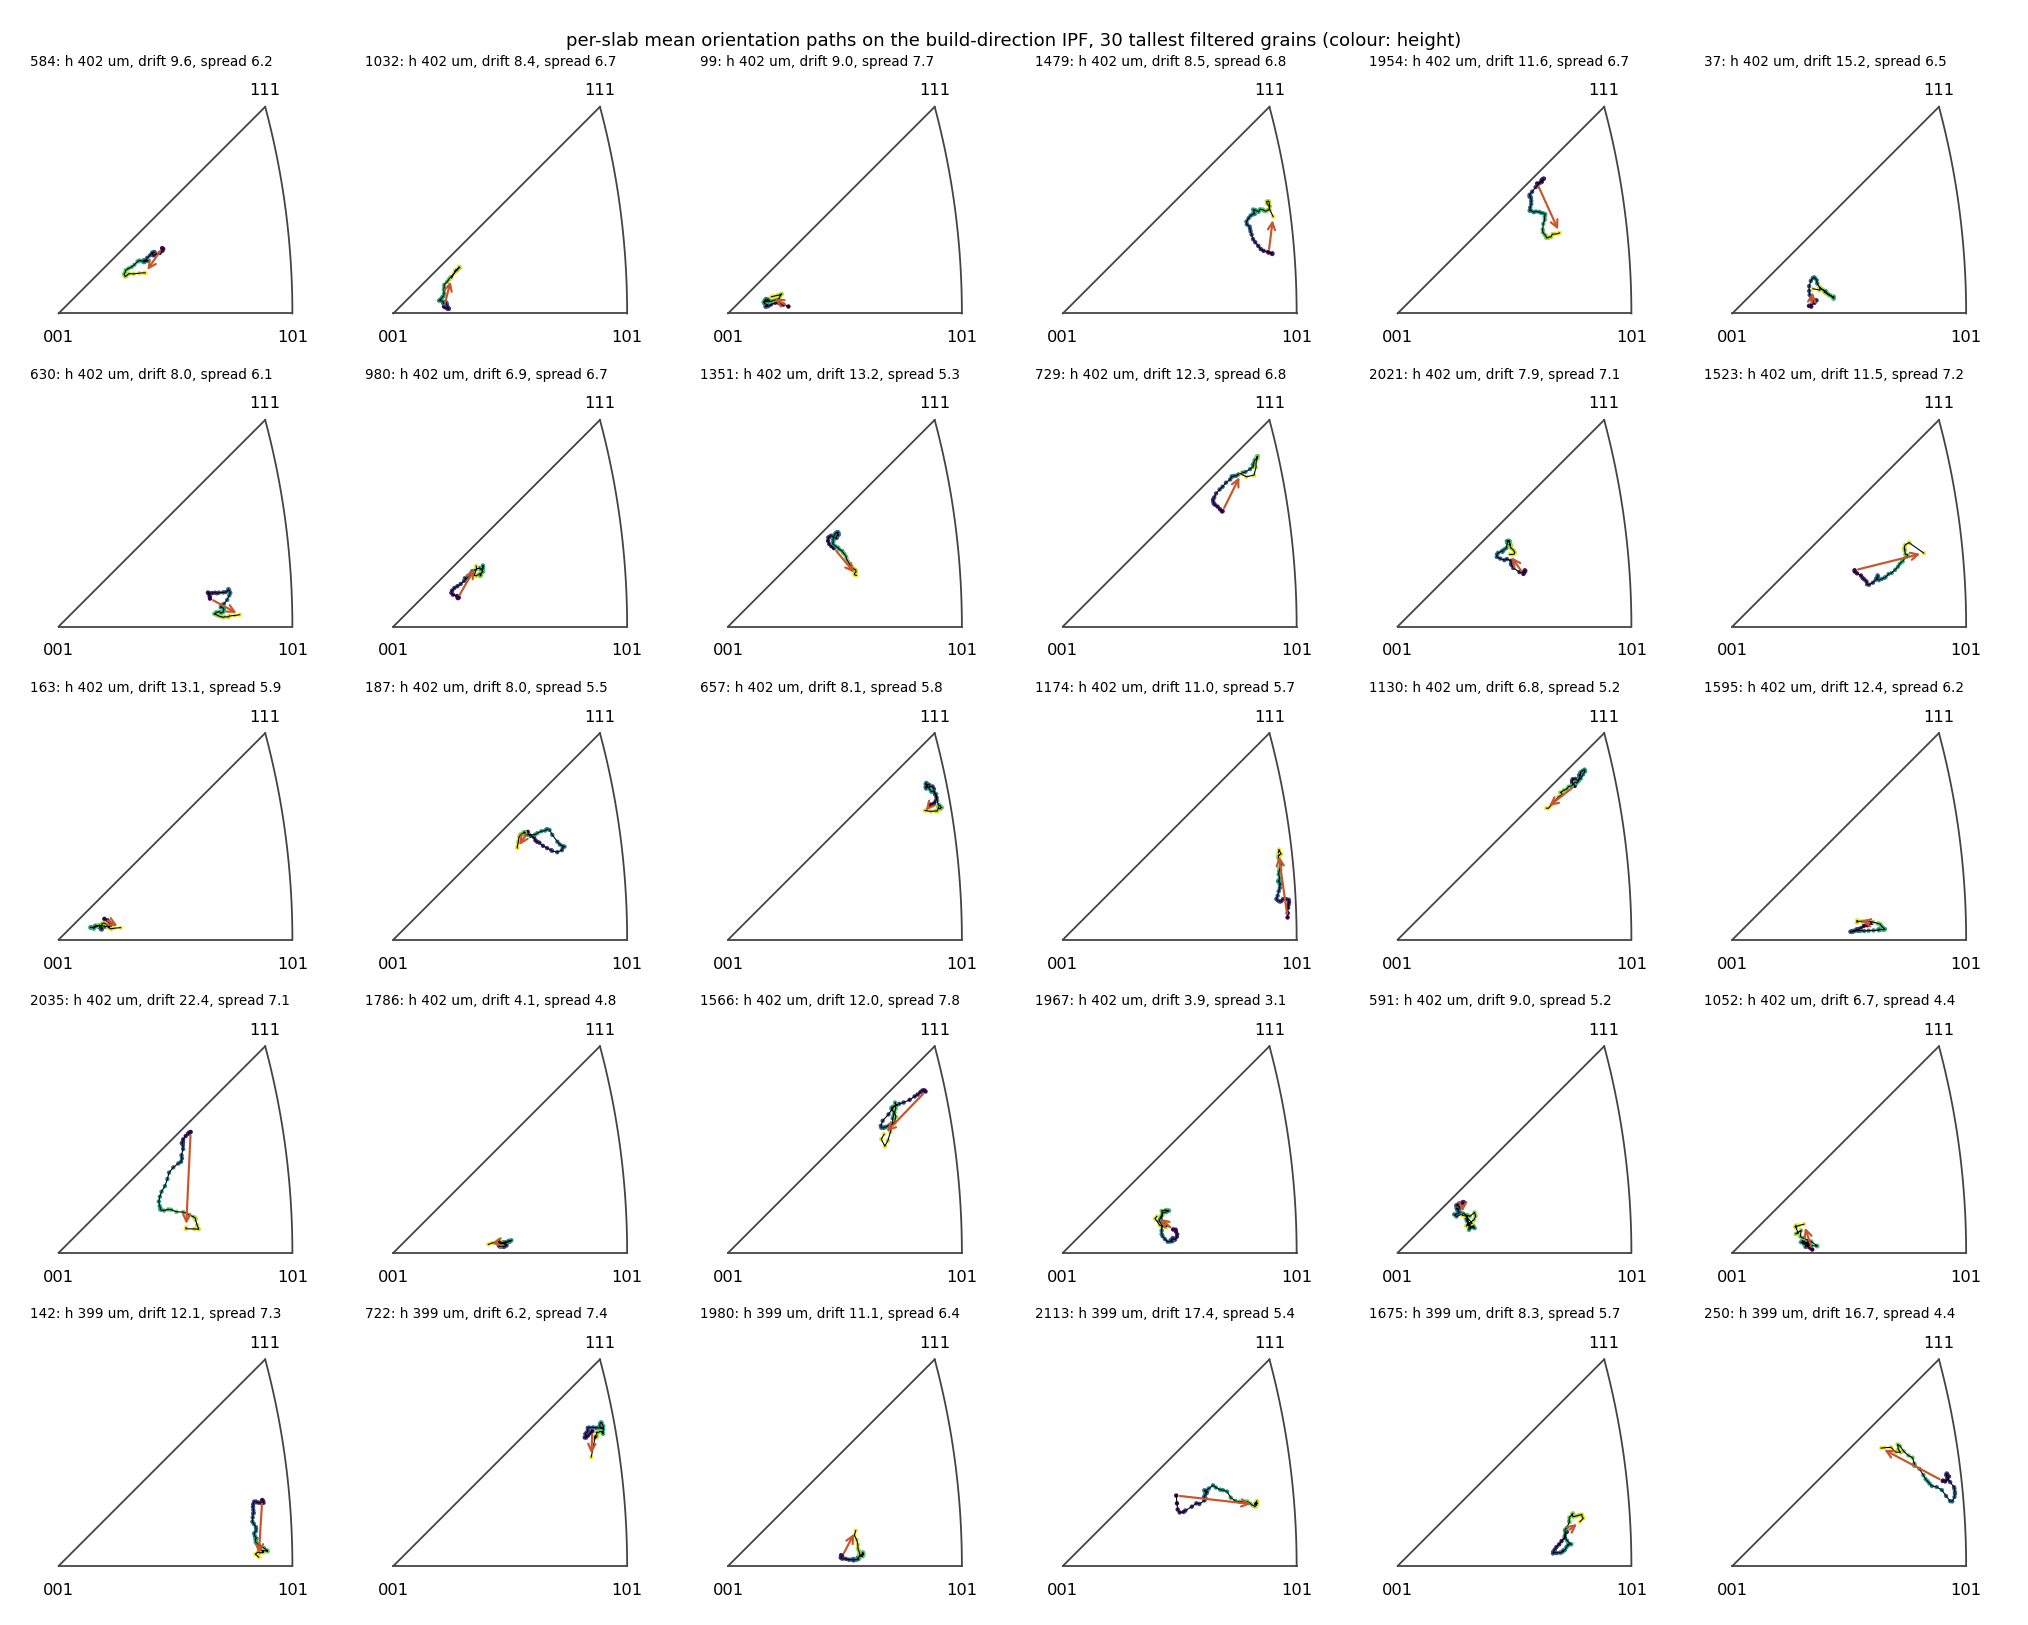
\includegraphics[width=\textwidth]{gp700_results_v10/grain_paths_grid.png}
\caption{v10: per-slab mean orientation of the 30 tallest filtered grains as paths on the build-direction inverse pole figure (colour: height; orange arrow: bottom to top).}
\label{fig:grid}
\end{figure}

\begin{figure}[htbp]
\centering
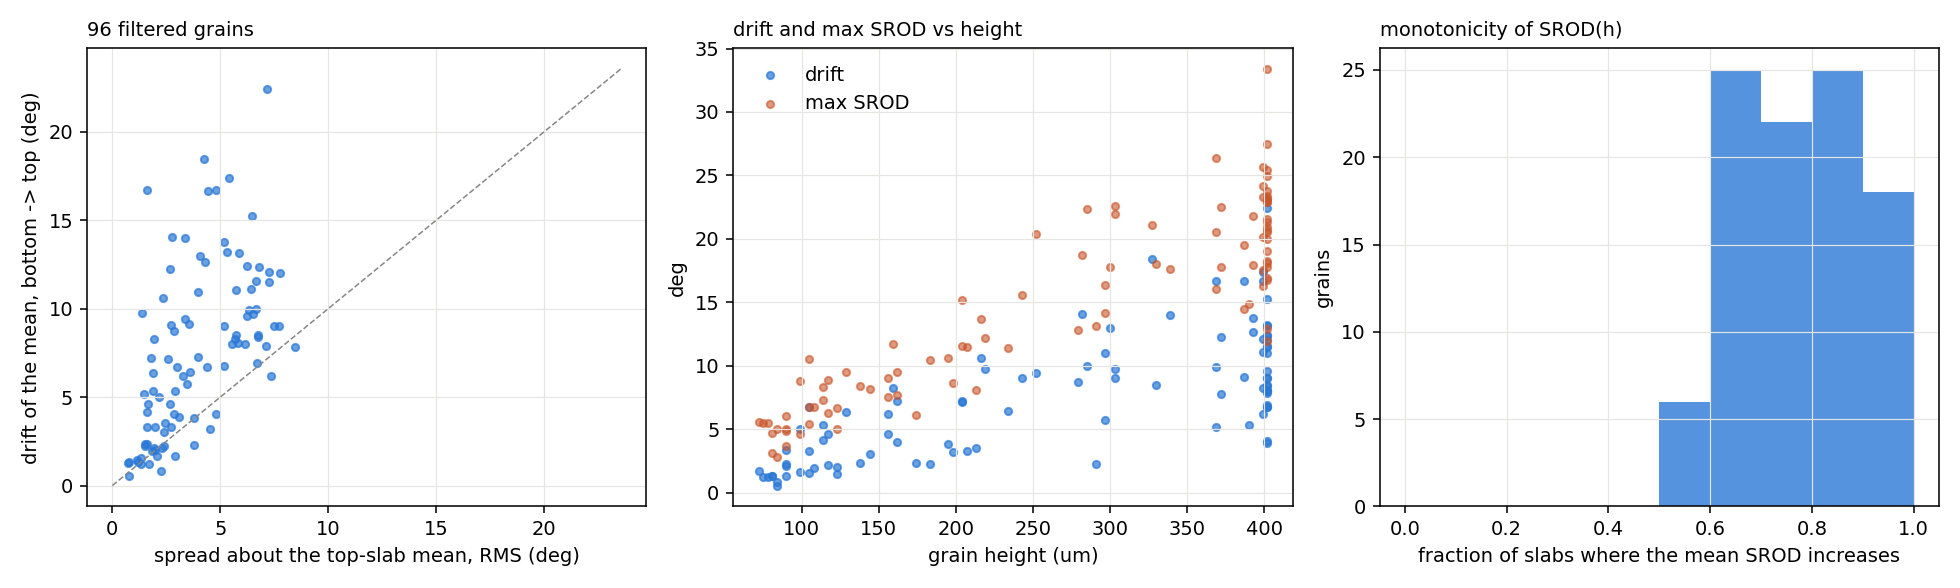
\includegraphics[width=\textwidth]{gp700_results_v10/grain_summary.png}
\caption{v10, all 96 filtered grains: drift against spread (dashed: equal), drift and maximum SROD against grain height, and the monotonicity of the per-grain SROD($h$).}
\label{fig:summary}
\end{figure}

In v10 the drift scales with grain height, about \SI{2}{\degree} at \SI{100}{\micro\metre} and 8--\SI{15}{\degree} at \SI{400}{\micro\metre}, nearly every grain drifts more than it spreads, and the tallest grains trace directed paths with maximum SROD of 20--\SI{24}{\degree}, the range Lamb report for their example grains. In v8 the grains spread more than they drift at every height. The two builds share the population level, band and maximum SROD, which is the point that the population statistics cannot separate the models while the per-grain ones can. The paths have no preferred direction on the triangle, as the isotropic rotation vector implies. About a fifth of the grains reverse over \SI{100}{\micro\metre} scales, which a \SI{30}{\micro\metre} correlation length allows.

\subsection{Resolution}
The per-voxel model (v8 deck) was run at Lamb's \SI{1.5}{\micro\metre} voxel on the proxy with the same $D$ and geometry: SROD RMS / bias \SI{0.49}{\degree} / \SI{+0.41}{\degree} against \SI{0.44}{\degree} / \SI{+0.03}{\degree} at \SI{3}{\micro\metre}, band 1.43 vs 1.41, same grain size and texture, with the finer lattice accumulating 10--18 \% more per unit height (retention against height 2.17 vs 1.83) because it resolves a slightly longer growth path. The per-hop rule is resolution independent to first order; an exact match at \SI{1.5}{\micro\metre} would take $D$ about 15 \% lower.

\subsection{Crop and grain origins}
Analysing v8 on the full \SI{801}{\micro\metre} domain, the central \SI{400}{\micro\metre}, the central \SI{200}{\micro\metre}, or with the never-remelted top layer removed changes the SROD bias by under \SI{0.2}{\degree} and the band by under 0.03. Of the 88 filtered grains in the standard crop, 83 originate at the layer-0 remelt floor (\SI{99}{\percent} of the filtered volume) and 3 above \SI{160}{\micro\metre}: the columnar grains are epitaxial continuations of substrate grains, so the simulated ``originating'' SROD is an established-grain SROD referenced at the remelt floor. Because Lamb's two classes share the same $D$, the walk comparison is unaffected, but the model does not generate Lamb's population of grains that originate mid-build.

\subsection{Texture}
Neither paper quantifies the \dir{001} fibre. A Sobol study over the mobility contrast $c_2$ and nucleation density with $D$ fixed gave \dir{001} within \SI{15}{\degree} of BD flat at 0.22 below $c_2 \approx 5$ and rising by 0.0125 per unit $c_2$ above it, with the SROD score unaffected; on the full build $c_2 = 9$ gave 0.22 against 0.19 at $c_2 = 2.8$. The coherent walk lowers the fraction further (v10: 0.15) because it carries grains out of the cone. The fraction is 1.7--2.5$\times$ random in every build.

\section{Findings and open issues}
\begin{enumerate}
\item Population SROD in GP700 is a rotation walk with $D \approx \SI{0.42}{\Dunit}$ against height and a Maxwell width; individual grains rotate coherently along a path.
\item The model reproduces both once orientation is inherited from one parent voxel and never averaged (per-grain parent selection, copy-mode smoothing) and a coherent, level-correlated grain walk is added to the per-voxel walk. The population statistics fix the total $D$; the per-grain drift-to-spread ratio fixes $D_g : D_v$; the shape of the individual curves and of the population curve below the correlation length fix $\rho$.
\item Deck constants are per unit of growth path, $1.8\times$ the height in this remelt geometry, and resolution independent to first order. Whether the real path factor is that large is an open physical question.
\item Grain classes do not match: no surviving grains originate mid-build at nucleation \SI{1.5e13}{\per\cubic\metre} with Lamb's filters, against their 5:1 originating-to-established ratio.
\item $D_g : D_v$ (Lamb's within-slice widths) and $\rho$ (their population curve below \SI{30}{\micro\metre}, the monotonicity of their grains) are constrained only loosely by the published figures; the direction of the per-grain paths on the inverse pole figure, isotropic in the model, is a further check available from their Fig.~4 data.
\item The \dir{001} fibre is twice random, moves weakly with the mobility contrast and falls with coherent rotation; there is no measured target.
\item Not yet tested: the undercooling dependence of $D_v$ ($\alpha > 0$).
\end{enumerate}

\section{Reproduction}
\begin{lstlisting}
. /home/tron/spack/share/spack/setup-env.sh && spack env activate spparks-dev
# binary: build-verify/spparks (commit 6a47de77 or later); template = the v10 deck
E=examples/gp700_moser; R=/home/tron/gp700_runs
$E/run_layers.sh build-verify/spparks $R/wide12_v10 12 12345 267 10 4e-6 $R/substrate_800um_50um_d10.st
/home/tron/miniconda3/envs/WORK/bin/python $E/gp700_analysis.py $R/wide12_v10/gp700.st \
    --out $R/wide12_v10/analysis_floor100 --floor-um 100 --crop 200 600 200 600
/home/tron/miniconda3/envs/WORK/bin/python $E/grain_paths.py $R/wide12_v10/gp700.st \
    --out $R/wide12_v10/grain_paths --crop 200 600 200 600 --floor-um 100 --grid 30
\end{lstlisting}
Runs live in \code{/home/tron/gp700\_runs/}. Key commits: fa8930f3 (per-voxel diffusion walk), ad23c1a5 (per-grain selection), 1a9712b3 (kk kernel parity), da2fad29 (\code{smooth\_orientation}), b6e4ba5f / 47546146 / 60b2d711 / 6a47de77 (\code{misorientation\_grain\_walk}: coherent walk, OU persistence, path index and d10, recurrence cache), f5d79cd3 (v10 deck). The development history with every intermediate run is in \code{docs/GP700\_MOSER\_SROD\_DECK\_PLAN.md}. This file is the reference version; \code{docs/SROD\_ANALYSIS\_REPORT.md} and the published HTML page mirror it.

\paragraph{Sources.} J.~Lamb et al., Acta Materialia (2023), 3D-EBSD and SROD of PBF-L GammaPrint-700; J.~Lamb et al., Metallurgical and Materials Transactions A (2026), cellular structure and 3DThesis parameters.
\end{document}
